\documentclass[11pt]{ctexart} 

%用来插入伪代码
\usepackage{algorithmicx}
\usepackage{algorithm}
\usepackage{algpseudocode}

%set A4 paper size and 1 inch margin
\usepackage[a4paper, margin=1in]{geometry} 

\usepackage{amsmath}

\usepackage{graphicx}


% 导入amsthm宏包,数学公式用
\usepackage{amsthm} 
% 支持一些数学符号,如 \mathbb
\usepackage{amssymb}

% 定义定理环境,插入定理用
\newtheorem{thm}{定理}
\newtheorem{gl}{公理}

% 超链接
\usepackage{hyperref}

% 允许为文字指定颜色或者高亮
\usepackage{xcolor}

%设置页眉页脚
\usepackage{fancyhdr}
\pagestyle{fancy}
\fancyhf{}
\fancyfoot[C]{\thepage}

% 参考文献样式(单独的.bib文件的引用方法)
\bibliographystyle{plain}%参考文献的样式

\title{机器人运动学}
\author{StuLiMing}
\date{} %取消显示日期

\begin{document}
\CJKindent                   %缩进
\maketitle                   %指明在这里生成文章的标题

\section{运动学}

\subsection{位置}

\subsubsection{点的相对位置}
点 B 相对于点A 的位置可以写成

\begin{equation}
    \mathbf{r_{AB}}
\end{equation}


\subsubsection{点在坐标系中的位置}
点在坐标系下的位置其实就是相对于坐标系 $\mathcal{A}$ 的原点 $A$ 的向量,表示为 ${\mathcal{A}}\mathbf{r}$

\noindent\textbf{笛卡尔坐标系}

\begin{equation}
    \left._\mathcal{A}\mathbf{r}=x\mathbf{e}_x^\mathcal{A}+y\mathbf{e}_y^\mathcal{A}+z\mathbf{e}_z^\mathcal{A}=\left(\begin{array}{c}x\\y\\z\end{array}\right.\right)
\end{equation}



\noindent\textbf{柱坐标}

\begin{equation}
    \left.\mathcal{A}\mathbf{r}=\left(\begin{array}{c}\rho\cos\theta\\\rho\sin\theta\\z\end{array}\right.\right)
\end{equation}


\noindent\textbf{球坐标}

球坐标系统使用三个坐标:径向距离($r$)、极角($\phi$)和方位角($\theta$)来描述一个点的位置。

径向距离($r$): 表示点到原点的直线距离。

极角($\phi$): 是从正z轴向下到点所在位置的射线与z轴之间的角度。$\phi\in (0,\pi)$.  

方位角($\theta$): 是从正x轴到点在xy平面上的投影与x轴之间的角度。


\begin{figure}[ht]
    \centering
    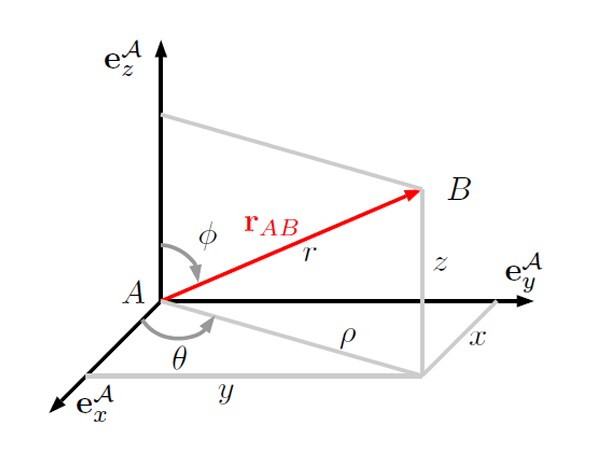
\includegraphics{images/1.jpg}
    \caption{ 使用笛卡尔、柱坐标和球坐标来表示位置}
    \label{label1}
\end{figure}

\begin{equation}
    \left.\mathcal{A}\mathbf{r}=\left(\begin{array}{c}r\cos\theta\sin\phi\\r\sin\theta\sin\phi\\r\cos\phi\end{array}\right.\right)
\end{equation}




\subsection{线速度}


\subsubsection{相对速度}
点 B 相对于点 A 的速度为:

\begin{equation}
    \dot{r}_{AB}
\end{equation}

这里加点表示对时间的导数。

在三维空间中,速度由向量 $\dot{r}\in \mathbb{R}^3$ 表示。

\subsubsection{线速度的表示}
$\chi_{P}$ 表示位置的堆积参数。即,在笛卡尔坐标系下
$$
\left.\chi_{P_c}=\left(\begin{array}{c}x\\y\\z\end{array}\right.\right)
$$
在柱坐标系下
$$
\left.\chi_{P_z}=\left(\begin{array}{c}\rho\\\theta\\z\end{array}\right.\right)
$$
在球坐标系下
$$
\left.\chi_{P_s}=\left(\begin{array}{c}r\\\theta\\\phi\end{array}\right.\right)
$$

速度 $\dot{r}$ 和当前形式下位置的导数 $\dot{\chi}_P$ 之间存在线性映射关系 $E_P(\chi)$:

\begin{equation}
    \dot{\mathbf{r}}=\mathbf{E}_{P}\left(\chi_{P}\right)\dot{\chi}_{P}
\end{equation}

\begin{equation}
    \dot{\chi}_{P}=\mathbf{E}_{P}^{-1}\left(\chi_{P}\right)\dot{\mathbf{r}}
\end{equation}

\noindent\textbf{笛卡尔坐标系}

如果采样笛卡尔坐标系,映射关系 $\mathbf{E}_{P}(\chi)$ 只是简单的单位矩阵
\begin{equation}
    \mathbf{E}_{P_c}\left(\boldsymbol{\chi}_{P_c}\right)=\mathbf{E}_{P_c}^{-1}\left(\boldsymbol{\chi}_{P_c}\right)=\mathbb{I}
\end{equation}

\noindent\textbf{柱坐标}
\begin{equation}
\left.\chi_{P_c}=\left(\begin{array}{c}x\\y\\z\end{array}\right.\right)=\left(\begin{array}{c}\rho\cos\theta\\\rho\sin\theta\\z\end{array}\right)
\end{equation}
从而
\begin{equation}
\dot{\chi}_{P_c}=\left(\begin{array}{c}\dot{x}\\\dot{y}\\\dot{z}\end{array}\right)=\left(\begin{array}{c}\dot{\rho}\cos\theta-\rho\dot{\theta}\sin\theta\\\dot{\rho}\sin\theta+\rho\dot{\theta}\cos\theta\\\dot{z}\end{array}\right)
=\begin{pmatrix}
    \cos\theta & -\rho\sin\theta & 0 \\
    \sin\theta & \rho\cos\theta & 0 \\
    0 & 0 & 1
    \end{pmatrix}\left(\begin{array}{c}\dot{\rho}\\\dot{\theta}\\\dot{z}\end{array}\right)=\mathbf{E}_{P}\left(\chi_{P}\right)
    \dot{\chi}_{Pz}
\end{equation}
从而
\begin{equation}
\mathbf{E}_{P}^{-1}=
\begin{pmatrix}
    cos\theta & sin\theta & 0 \\
    -sin\theta/\rho & cos\theta/\rho & 0 \\
    0 & 0 & 1 \\
\end{pmatrix}
\end{equation}

\noindent\textbf{球坐标}

类似地
\begin{equation}
\dot{\boldsymbol{\chi}}_{P_{c}}=\left(\begin{array}{c}{\dot{x}}\\{\dot{y}}\\{\dot{z}}\end{array}\right)=\left(\begin{array}{c}{\dot{r}\cos\theta\sin\phi-r\dot{\theta}\sin\theta\sin\phi+r\dot{\phi}\cos\theta\cos\phi}\\{\dot{r}\sin\theta\sin\phi+r\dot{\theta}\cos\theta\sin\phi+r\dot{\phi}\sin\theta\cos\phi}\\{\dot{r}\cos\phi-r\dot{\phi}\sin\phi}\end{array}\right) 
\end{equation}
从而
\begin{equation}
\begin{gathered}
    \mathbf{E}_{Ps}= \left(\begin{array}{ccc}\cos\theta\sin\phi&-r\sin\phi\sin\theta&r\cos\phi\cos\theta\\\sin\phi\sin\theta&r\cos\theta\sin\phi&r\cos\phi\sin\theta\\\cos\phi&0&-r\sin\phi\end{array}\right) \\
    \mathbf{E}_{Ps}^{-1}= \left(\begin{array}{ccc}\cos\theta\sin\phi&\sin\phi\sin\theta&\cos\phi\\-\sin\theta/(r\sin\phi)&\cos\theta/(r\sin\phi)&0\\(\cos\phi\cos\theta)/r&(\cos\phi\sin\theta)/r&-\sin\phi/r\end{array}\right) 
\end{gathered}
\end{equation}

\subsection{旋转}
\subsubsection{姿态}
为了描述物体的姿态,在物体上固定一个坐标系并且给出此坐标系相对于参考坐标系的描述。假设世界坐标系是 $\mathcal{A}$, 物体的坐标系是 $\mathcal{B}$ 那物体的姿势可以被 3x3 矩阵
\begin{equation}
\left[ _Ae_z^{\mathcal{B}}\,\,, _Ae_y^{\mathcal{B}},\, _Ae_z^{\mathcal{B}} \right] 
\end{equation}
描述。

考虑 $\mathcal{A}$ 和 $\mathcal{B}$ 原点重合的情形:
\begin{equation}
_{\mathcal{A}}\mathbf{r}_{AP}={}_{\mathcal{A}}\mathbf{e}_{x}^{\mathcal{B}}\cdot_{\mathcal{B}}r_{AP_{x}}+{}_{\mathcal{A}}\mathbf{e}_{y}^{\mathcal{B}}\cdot{}_{\mathcal{B}}r_{AP_{y}}+{}_{\mathcal{A}}\mathbf{e}_{z}^{\mathcal{B}}\cdot{}_{\mathcal{B}}r_{AP_{z}}
\end{equation}
或者

\begin{equation}
\begin{aligned}
    _{\mathcal{A}}\mathbf{r}_{AP}& \left.=\left[\begin{array}{ccc}{{_{\mathcal{A}}\mathbf{e}_{x}^{\mathcal{B}}}}&{{_{\mathcal{A}}\mathbf{e}_{y}^{\mathcal{B}}}}&{{_{\mathcal{A}}\mathbf{e}_{z}^{\mathcal{B}}}}\\\end{array}\right.\right]\cdot\mathcal{B}\mathbf{r}_{AP}  \\
    &=\mathbf{C}_{\mathcal{AB}}\cdot{}_{\mathcal{B}\mathbf{r}_{AP}}
    \end{aligned}
\end{equation}

$\mathbf{C}_{\mathcal{A}\mathcal{B}}$ 项被称为旋转矩阵,是一个 3x3 矩阵。

$\mathbf{C}_{\mathcal{A}\mathcal{B}}$ 是正交的,意味着:
1. $\mathbf{C}_{\mathcal{AB}}^T\cdot\mathbf{C}_{\mathcal{AB}}=\mathbb{I}_3$

$\mathbf{C}_{\mathcal{A}\mathcal{B}}$ 同样构成描述旋转的矩阵,无论这个旋转是物体主动完成的,还是某种坐标系的变换。


这里注意下 $\mathbf{C}_{\mathcal{A}\mathcal{B}}$ 下标是先 $\mathcal{A}$ 后 $\mathcal{B}$,意思是 $\mathcal{A}$ 坐标系下 $\mathcal{B}$ 的基向量的矩阵,但是效果却是将 $\mathcal{B}$ 坐标系下的坐标转换为 $\mathcal{A}$ 坐标系下的坐标。

\subsubsection{基础旋转}
\textbf{基础旋转}是围绕坐标系的三个正交基向量中的任何一个的旋转,给定坐标轴,基础旋转只有一个参数:旋转角度 $\varphi$

三个基础旋转分别是:
\begin{equation}
{\bf C}_{x}(\varphi)=\left[\begin{array}{c c c}{{1}}&{{0}}&{{0}}\\ {{0}}&{{\mathrm{cos}\,\varphi}}&{{-\mathrm{sin}\,\varphi}}\\ {{0}}&{{\mathrm{sin}\,\varphi}}&{{\mathrm{cos}\,\varphi}}\end{array}\right]
\end{equation}
\begin{equation}
{\bf C}_{y}(\varphi)=\left[\begin{array}{c c c}{{\mathrm{cos}\,\varphi}}&{{0}}&{{\mathrm{sin}\,\varphi}}\\ {{0}}&{{1}}&{{0}}\\ {{-\mathrm{sin}\,\varphi}}&{{0}}&{{\mathrm{cos}\,\varphi}}\end{array}\right].
\end{equation}
\begin{equation}
{\bf C}_{z}(\varphi)=\left[\begin{array}{c c c}{{\cos\varphi}}&{{-\sin\varphi}}&{{0}}\\ {{\sin\varphi}}&{{\cos\varphi}}&{{0}}\\ {{0}}&{{0}}&{{1}}\end{array}\right]
\end{equation}

这很显然:
\begin{figure}[ht]
    \centering
    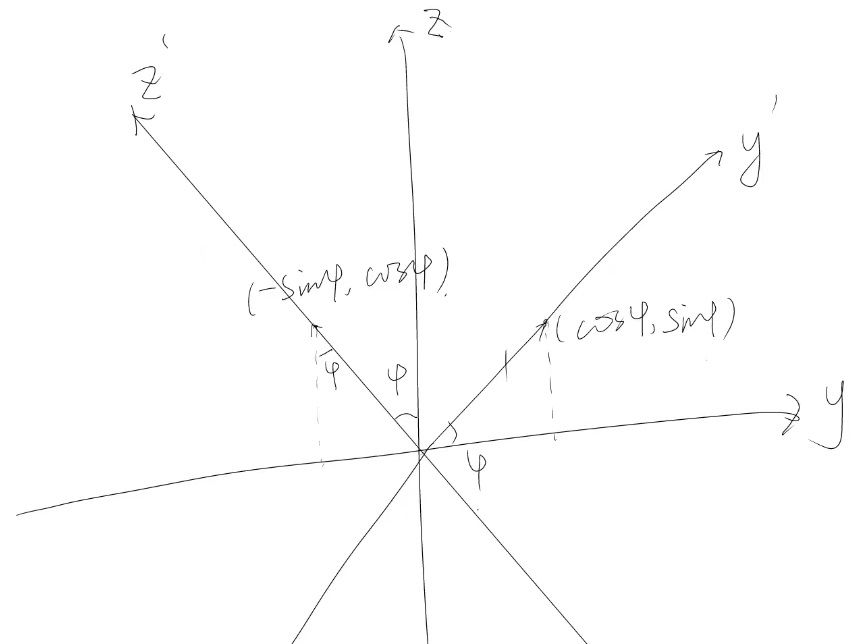
\includegraphics[scale=0.75]{images/2.jpg}
    \caption{基础旋转的简单推导}
    \label{label2}
\end{figure}

1. 注意旋转操作是非交换的(用一个魔方试一下就很显然了)。
2. 只要三个参数就可以表示一个旋转

\subsubsection{旋转表示}

\noindent\textbf{欧拉角}
用三次基础旋转的复合表示一个一般的旋转

下面主要介绍 ZYZ 欧拉角。
\begin{figure}[ht]
    \centering
    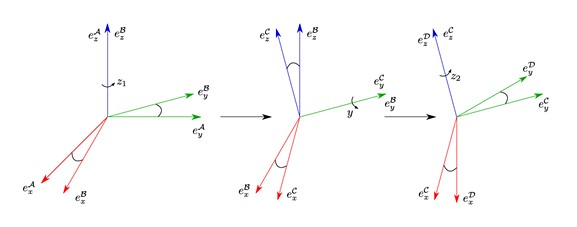
\includegraphics{images/3.jpg}
    \caption{ZYZ欧拉角}
    \label{label3}
\end{figure}

\begin{equation}
    \begin{split}
        \mathbf{C}_{A D} &= \mathbf{C}_{A B}\left(z_{1}\right)\mathbf{C}_{B C}\left(y\right)\mathbf{C}_{C D}\left(z_{2}\right) \\
        &\Rightarrow A\mathbf{r} = \mathbf{C}_{A D D}\mathbf{r} \\
        &= \left[\begin{array}{ccc}\cos z_1&-\sin z_1&0\\\sin z_1&\cos z_1&0\\0&0&1\end{array}\right]
        \left[\begin{array}{ccc}\cos y&0&\sin y\\0&1&0\\-\sin y&0&\cos y\end{array}\right]
        \left[\begin{array}{ccc}\cos z_2&-\sin z_2&0\\\sin z_2&\cos z_2&0\\0&0&1\end{array}\right] \\
        &= \left[\begin{array}{ccc}
        c_yc_{z_1}c_{z_2}-s_{z_1}s_{z_2}&-c_{z_2}s_{z_1}-c_yc_{z_1}s_{z_2}&c_{z_1}s_y \\
        c_{z_1}s_{z_2}+c_yc_{z_2}s_{z_1}&c_{z_1}c_{z_2}-c_ys_{z_1}s_{z_2}&s_ys_{z_1} \\
        -c_{z_2}s_y&s_ys_{z_2}&c_y
        \end{array}\right]
    \end{split}
    \end{equation}

这里 c 和 s 是 cos 和 sin 的简写。

给定矩阵
\begin{equation}
{\bf C}_{A D}=\left[\begin{array}{c c c}{{c_{11}}}&{{c_{12}}}&{{c_{13}}}\\ {{c_{21}}}&{{c_{22}}}&{{c_{23}}}\\ {{c_{31}}}&{{c_{32}}}&{{c_{33}}}\end{array}\right]
\end{equation}
可以反解出欧拉角
\begin{equation}
    \left.\chi_{R\text{euler}ZYZ}=\left(\begin{array}{c}z_{1}\\y\\z_{2}\end{array}\right.\right)=\left(\begin{array}{c}\operatorname{atan}2\left(c_{23}c_{13}\right)\\\operatorname{atan}2\left(\sqrt{c_{13}^2+c_{23}^2}c_{33}\right)\\\operatorname{atan}2\left(c_{32}-c_{31}\right)\end{array}\right)
\end{equation}
    
除此之外,还有 ZXZ 欧拉角、ZYX 欧拉角、XYZ 欧拉角。

\noindent\textbf{轴角}
轴角是由角度 $\theta$ 和旋转轴 $\bf{n}$ 定义的非最小参数化表示旋转的方法。向量 $\bf{n}\in\mathbb{R}^3$ 定义旋转的方向,而标量 $\theta\in\mathbb{R}$ 定义旋转角度:

\begin{equation}
    \left.\chi_{R\text{Angle Axis}}=\left(\begin{array}{c}\theta\\\mathbf{n}\end{array}\right.\right)
\end{equation}




























\end{document}